\section{DRIFT: Claim-Centric Trajectory Auditing}

\paragraph{Motivation and formulation.}
After trajectory collection, span segmentation, and error span annotation, we introduce \textsc{DRIFT} to localize erroneous spans in a completed trajectory. Given a task question $q$ and an ordered span sequence $T=(s_1,\ldots,s_n)$, \textsc{DRIFT} predicts a set of error spans $\hat{E}\subseteq T$:
\begin{equation}
    \hat{E}=f_{\theta}(q,T).
    \label{eq:drift-task}
\end{equation}
The external input contains only the question and raw span text; it does not use judge results, gold labels, manual notes, span types, or generated summaries. The key design choice is to audit claims rather than classify spans independently. In deep-research trajectories, many spans are exploratory: an agent searches, tests candidates, follows weak leads, and may later abandon them. Such spans are not harmful by themselves. A span becomes harmful when the agent commits to an unsupported, conflicting, or prematurely finalized claim and later reasoning treats that claim as established. Thus, \textsc{DRIFT} localizes errors through the claim-centric workflow in Figure~\ref{fig:overview}: when a claim is introduced, whether it is supported, and where it becomes consequential for the answer path.
\begin{figure*}[!t]
  \centering
  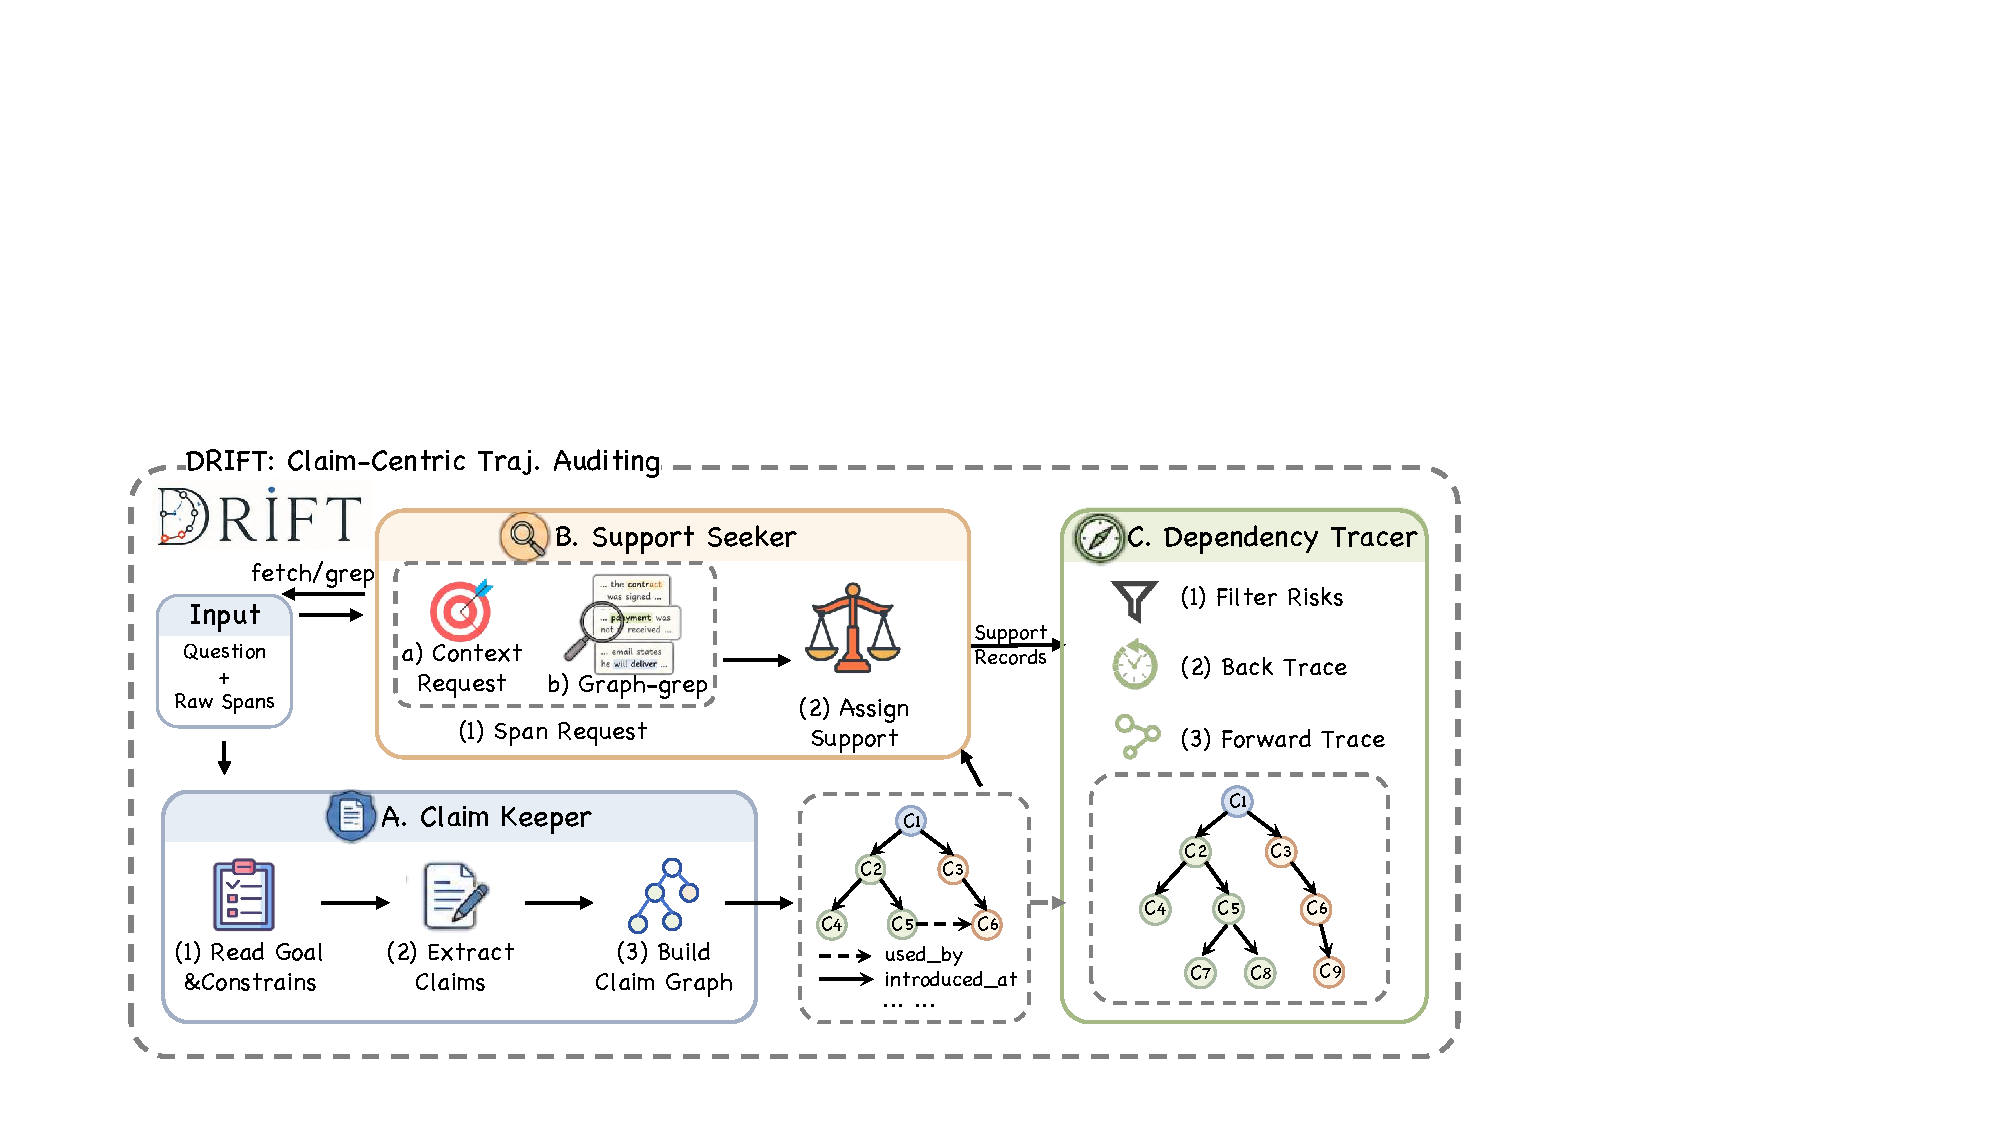
\includegraphics[width=1\textwidth]{figure/agenterr_1_.pdf}
  \caption{Overview of \textsc{DRIFT}: a claim-centric auditing workflow that builds trajectory-level claim ledgers, verifies support, and traces claim dependencies to localize first and follow-up errors.}
  \label{fig:overview}
\end{figure*}
\paragraph{A: Claim Keeper.}
\textsc{DRIFT} first performs a global pass over the full ordered trajectory to construct a claim ledger. A claim is a decision-relevant belief or commitment made by the agent, such as selecting an entity, accepting a constraint, interpreting evidence, relying on retrieval coverage, completing a computation, or deciding that no answer can be produced. For each claim, the ledger records where it is introduced, where it first becomes consequential, which later spans reuse it, its claim type, and its commitment status. We write the ledger as
\begin{equation}
    \mathcal{L}=\{c_k\}_{k=1}^{m},
    \qquad
    c_k=(a_k,i_k,b_k,U_k,\tau_k,\sigma_k).
    \label{eq:claim-ledger}
\end{equation}
Here, $a_k$ is the textual claim, $i_k$ is the span where it is introduced, $b_k$ is the first span where it becomes consequential, $U_k$ is the set of later spans that use it, $\tau_k$ denotes the claim type, and $\sigma_k$ denotes its status, such as exploratory, tentative, consequential, or finalized. This ledger separates ordinary exploration from committed reasoning: a candidate name in a query is only exploratory, whereas using that candidate as a settled premise is consequential.


\paragraph{B: Support Seeker.}
Given the claim ledger, the Support Seeker checks whether each consequential claim is supported by evidence shown in the trajectory. It assigns one of four support statuses: \textsc{direct}, \textsc{weak}, \textsc{missing}, or \textsc{conflicting}. \textsc{direct} means that the trajectory directly establishes the decisive link needed by the claim; \textsc{weak} means that related evidence exists but the decisive link is partial, implicit, snippet-based, or unchecked; \textsc{missing} means that no shown support establishes the claim; and \textsc{conflicting} means that shown evidence contradicts the claim. The Support Seeker also records the spans that provide or fail to provide support. Importantly, this stage does not output final error spans. Its role is to expose support risks for claims that may later become harmful commits.

\paragraph{C: Dependency Tracer.}
The final Dependency Tracer takes the claim ledger and support records, then determines which risky claims correspond to harmful error spans. A weak or missing support record is not sufficient by itself: the tracer must identify whether the claim is used as a commitment, propagated into later reasoning, computed from, used to give up, or finalized in the answer. \textsc{DRIFT} marks as error the spans that commit to, reuse, amplify, or finalize unsupported or conflicting consequential claims, and marks the remaining spans as non-error.

The final prediction is a set of error spans:
\begin{equation}
    \hat{E}=\{s_j \in T \mid h(s_j)=1\},
    \label{eq:final-prediction}
\end{equation}
where $h(s_j)=1$ indicates that span $s_j$ commits to, reuses, amplifies, or finalizes a harmful claim.






